\section{Additional Details on Software Outputs and Functionality}\label{sec:additional-outputs}

The \texttt{GLaRe()} summary plot is the default graphic returned by the \proglang{GLaRe()} function (Figure \ref{fig:glare-anatomy-plot}).
The overall, or average, cross-validated loss is displayed in yellow, with the analogous loss computed on the training data shown in green for comparison.
Then, different quantiles of the distribution of individual cross-validated losses are displayed to summarize the full distribution: the minimum and maximum are shown in blue and red, respectively, a user-specified quantile of the distribution (set by the \texttt{cvqlines} argument) is displayed in purple and the quantile of the distribution being used as the attainment rate $\alpha$ (defaulting to 0.95, i.e., the $95$th percentile) is displayed in light gray.
The corresponding value of the tolerance level $\epsilon$ is overlaid as gray dashed horizontal line, and hence the latent feature dimension (i.e., location on the $x$-axis) at which the two gray lines meet corresponds to the qualifying dimension.
The tolerance level $\epsilon$ and the qualifying dimension ($qd$) are marked in bold and italic typeface on the $y$ and $x$ axes, respectively.
The \texttt{GLaRe()} function also returns a heat-map as an alternative summary of the individual cross-validated loss distribution, and the package also contains wrapper functions to display a dot-plot of the full distribution of cross-validated losses, the ratio of training to cross-validated losses and the reconstructions of individual observations at the qualifying dimension. 

\begin{figure}
    \centering
    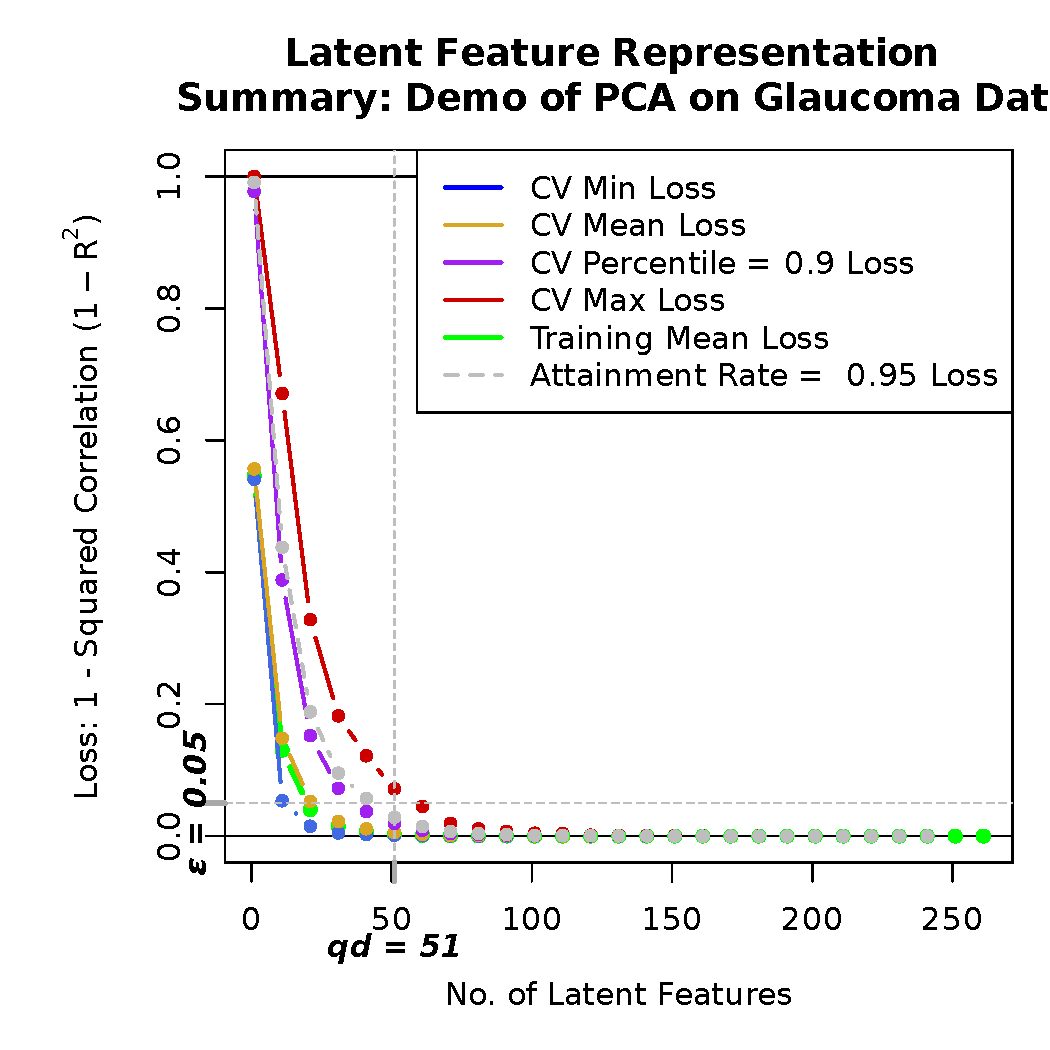
\includegraphics[width=0.5\linewidth]{figures/glare-anatomy-plot.pdf}
    \caption{The summary plot produced by \texttt{GlaRe()}, demonstrated on the Glaucoma dataset with PCA.}
    \label{fig:glare-anatomy-plot}
\end{figure}

The \texttt{GLaRe()} function also returns a heatmap to display the full distribution of generalization errors (Figure \ref{fig:eye-heatmap}).
It is obtained by re-ordering the $N$ values within each column of the matrix of cross-validated information losses.
The latent feature dimension is represented on the $x$-axis, the corresponding quantile of the generalization error distribution at that feature dimension (i.e., column) is shown on the $y$-axis and the color represents the value of the generalization error at that feature dimension and quantile.


\begin{figure}
    \centering
    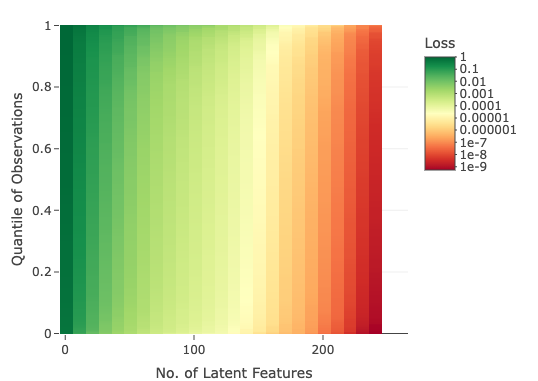
\includegraphics[width=0.5\linewidth]{figures/eye-heatmap.png}
    \caption{The heatmap returned by \texttt{GLaRe()} used to summarize the full distribution of generalization errors (i.e., cross-validated estimates of information loss). The latent feature dimension is represented on the $x$-axis, the corresponding quantile of the generalization error distribution at that feature dimension is shown on the $y$-axis and the color represents the value of the generalization error at that feature dimension and quantile.}
    \label{fig:eye-heatmap}
\end{figure}

The \pkg{GLaRe} package also contains wrapper functions that plot alternative summaries of the cross-validated distribution of information losses; their outputs are displayed in Figure \ref{fig:additional-plots-01}.
The function \texttt{distribution\_plot()} produces a dot-plot of the individual cross-validated information loss distribution, where each point represents an individual value and the points are colored according to the latent feature dimension $K$ (Figure \ref{fig:additional-plots-01} \textbf{(a)}).

\begin{figure}
    \centering
    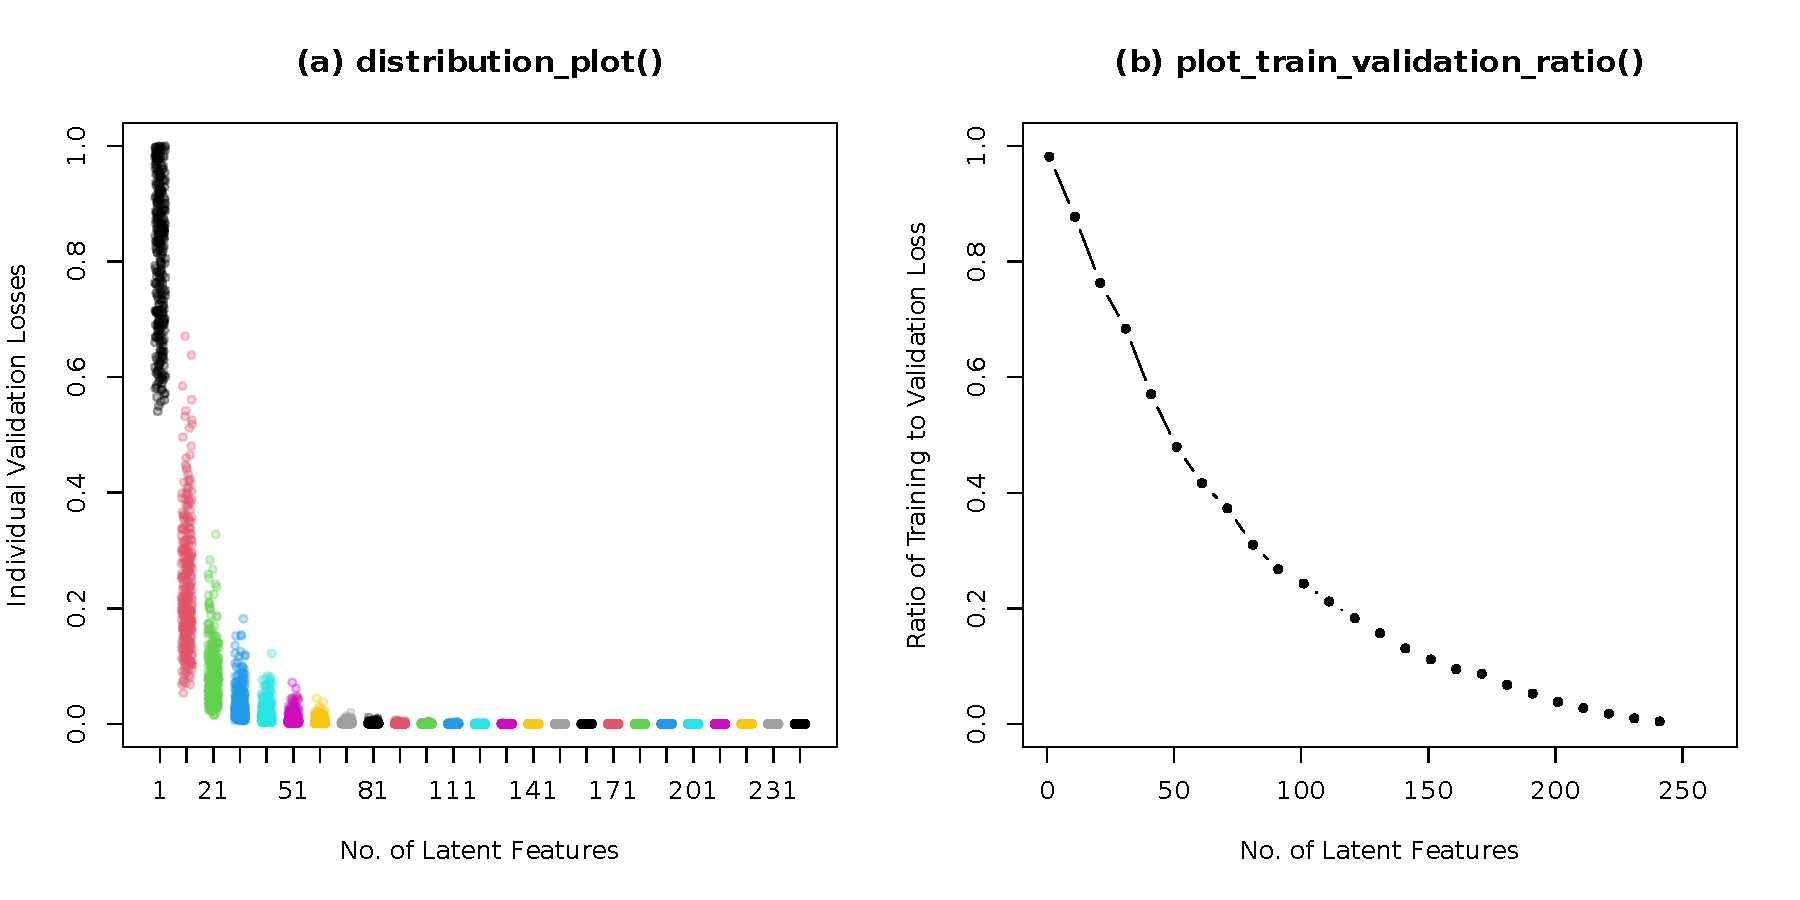
\includegraphics[width=1\linewidth]{figures/additional-plots-01.pdf}
    \caption{Additional wrapper functions that produce summary plots of \texttt{GLaRe()} outputs. \textbf{(a)} \texttt{distribution\_plot()} produces a dot-plot of the individual cross-validated information loss distribution. \textbf{(b)} \texttt{plot\_train\_validation\_ratio()} produces a point and line plot of the ratio of the total training and validation losses.
    Both plots are demonstrated on the Glaucoma dataset with a PCA representation from Section \ref{sec:software}.}
    \label{fig:additional-plots-01}
\end{figure}

When the qualifying criterion is met, the CLaRe framework fits the final model on the full dataset at the qualifying dimension.
The \pkg{GLaRe} package contains functions to visually inspect the reconstruction of individual observations from the final model.
Due to the non-standard structure of the Glaucoma, Proteomic Gels and MNIST data, we have written custom functions to display side-by-side plots of the data observation and its reconstruction (Figures \ref{fig:eye-reconstruction} -- \ref{fig:mnist-reconstruction}).
For data objects which are $1$-dimensional signals, we provide a general function called \texttt{plot\_1D\_reconstruction()} that displays the original signal as a solid line and overlays its reconstruction as a dotted line (Figure \ref{fig:phoneme-reconstruction}).
Unlike the specialized functions that plot side-by-side plots, this function can display the reconstruction of more than one observation simultaneously.

\begin{figure}
    \centering
    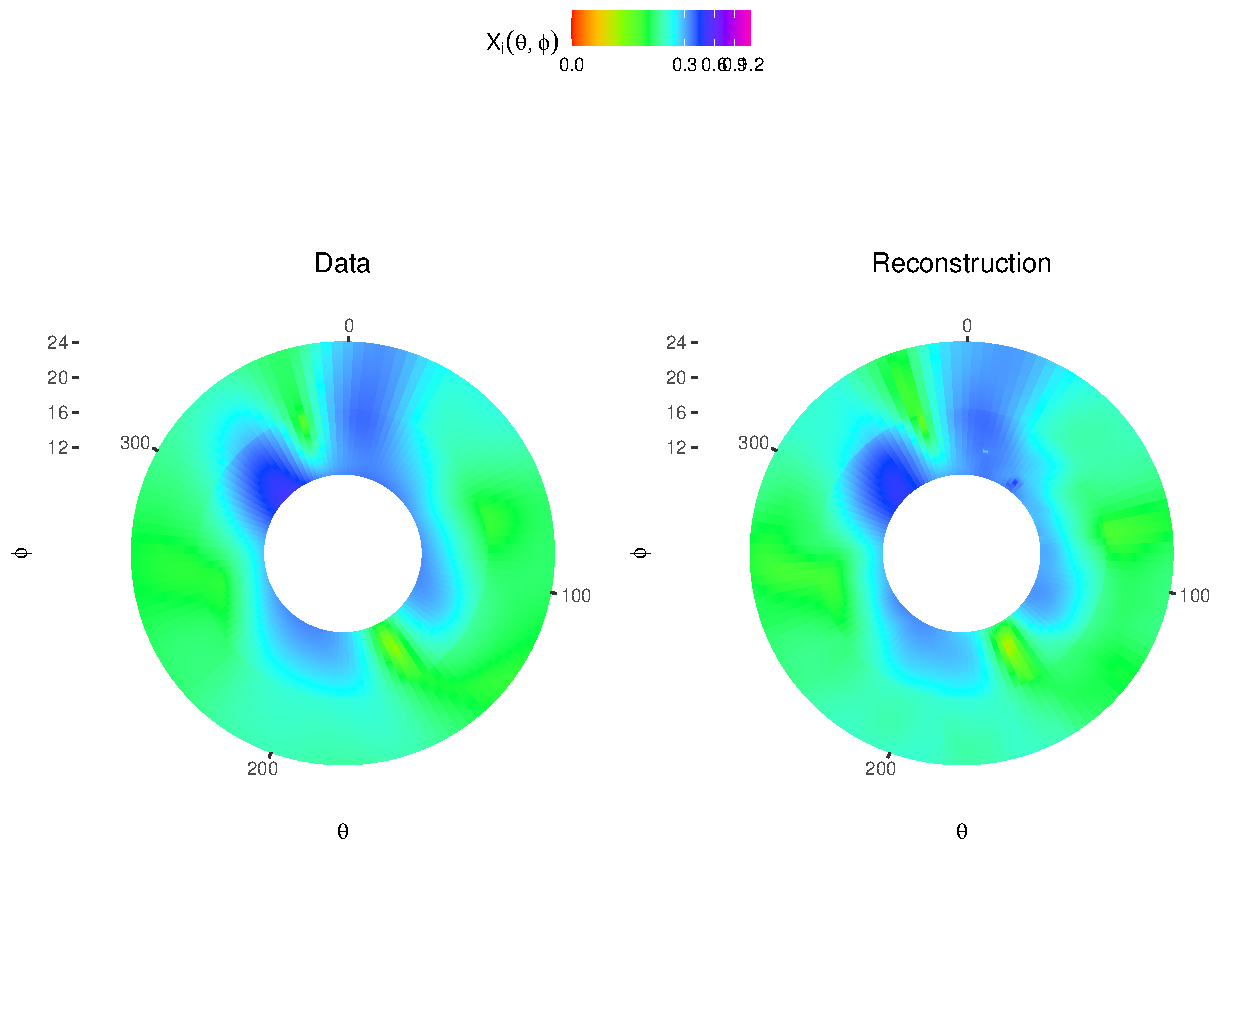
\includegraphics[width=0.75\linewidth]{figures/eye-reconstruction.pdf}
    \caption{A single observation from the Glaucoma data (left) and its reconstruction (right) using the final model fit from PCA at the qualifying dimension $qd = 51$. The figure was generated using the \texttt{plot\_eye\_reconstruction()} function from the \pkg{GLaRe} package. A cubed-root transformation is applied for visualization.}
    \label{fig:eye-reconstruction}
\end{figure}

\begin{figure}
    \centering
    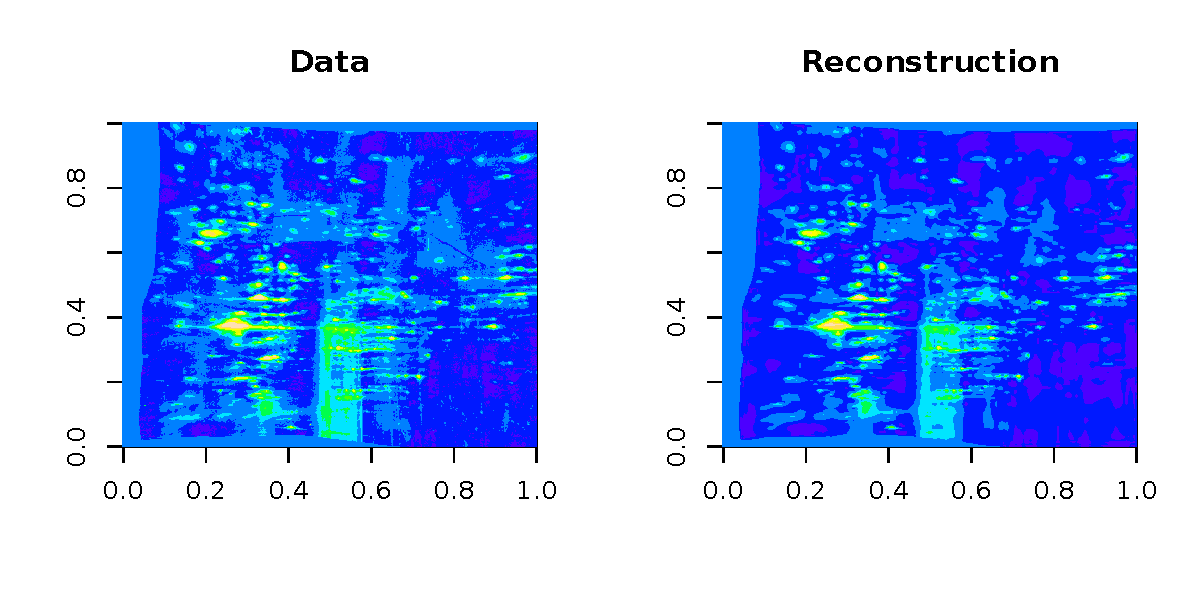
\includegraphics[width=0.75\linewidth]{figures/gels-reconstruction.pdf}
    \caption{A single observation from the Proteomic Gels data (left) and its reconstruction (right) using the final model fit from DWT at the qualifying dimension $qd = 7801$. The figure was generated using the \texttt{plot\_gels\_reconstruction()} function from the \pkg{GLaRe} package.}
    \label{fig:gels-reconstruction}
\end{figure}

\begin{figure}
    \centering
    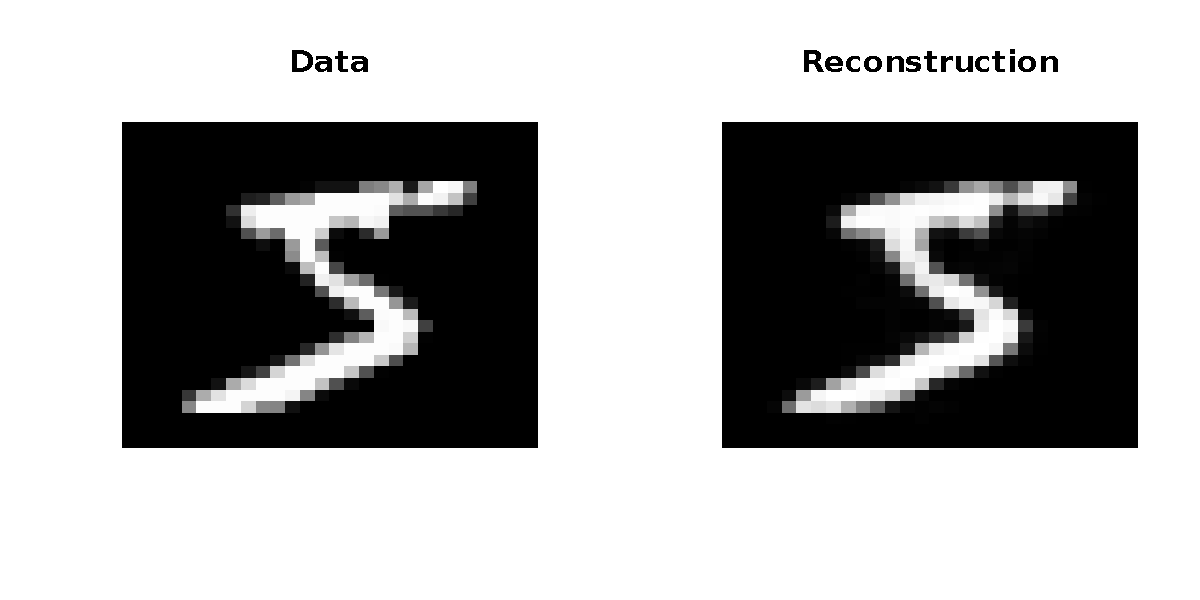
\includegraphics[width=0.75\linewidth]{figures/mnist-reconstruction.pdf}
    \caption{A single observation from the MNIST Digits data (left) and its reconstruction (right) using the final model fit from AE at the qualifying dimension $qd = 101$. The figure was generated using the \texttt{plot\_mnist\_reconstruction()} function from the \pkg{GLaRe} package.}
    \label{fig:mnist-reconstruction}
\end{figure}

\begin{figure}
    \centering
    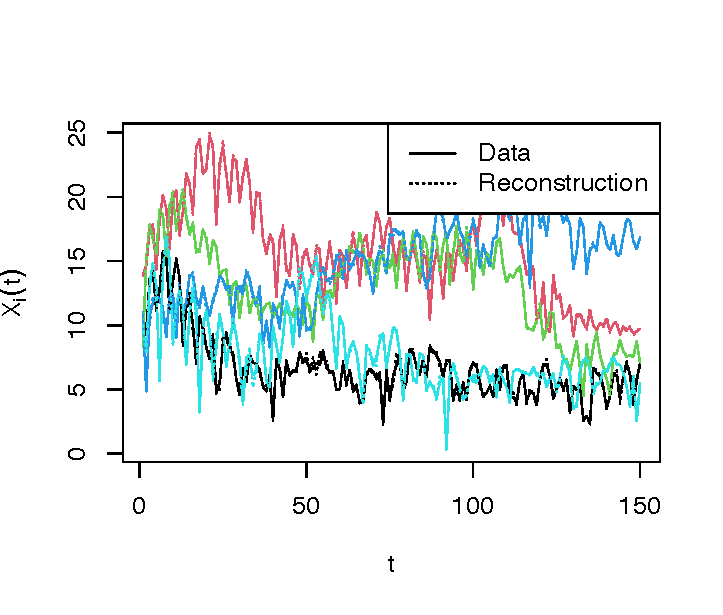
\includegraphics[width=0.75\linewidth]{figures/phoneme-reconstruction.pdf}
    \caption{Reconstructions of $8$ observations from the \texttt{phenome} dataset (dotted lines) overlaid on the original observations (solid lines). The reconstructions were computed from the final model fit of PCA at the qualifying dimension $qd=126$. The figure was generated using the \texttt{plot\_1D\_reconstruction()} function from the \pkg{GLaRe} package.}
    \label{fig:phoneme-reconstruction}
\end{figure}